\documentclass[11pt,a4paper]{report}
\usepackage[textwidth=37em,vmargin=30mm]{geometry}
\usepackage{calc,xunicode,amsmath,amssymb,paralist,enumitem,tabu,booktabs,datetime2,xeCJK,xeCJKfntef,listings}
\usepackage{tocloft,fancyhdr,tcolorbox,xcolor,graphicx,eso-pic,xltxtra,xelatexemoji}

\newcommand{\envyear}[0]{2024}
\newcommand{\envdatestr}[0]{2024-10-27}
\newcommand{\envfinaldir}[0]{webdb/2024/20241027/final}

\usepackage[hidelinks]{hyperref}
\hypersetup{
    colorlinks=false,
    pdfpagemode=FullScreen,
    pdftitle={Web Digest - \envdatestr}
}

\setlength{\cftbeforechapskip}{10pt}
\renewcommand{\cftchapfont}{\rmfamily\bfseries\large\raggedright}
\setlength{\cftbeforesecskip}{2pt}
\renewcommand{\cftsecfont}{\sffamily\small\raggedright}

\setdefaultleftmargin{2em}{2em}{1em}{1em}{1em}{1em}

\usepackage{xeCJK,xeCJKfntef}
\xeCJKsetup{PunctStyle=plain,RubberPunctSkip=false,CJKglue=\strut\hskip 0pt plus 0.1em minus 0.05em,CJKecglue=\strut\hskip 0.22em plus 0.2em}
\XeTeXlinebreaklocale "zh"
\XeTeXlinebreakskip = 0pt


\setmainfont{Brygada 1918}
\setromanfont{Brygada 1918}
\setsansfont{IBM Plex Sans}
\setmonofont{JetBrains Mono NL}
\setCJKmainfont{Noto Serif CJK SC}
\setCJKromanfont{Noto Serif CJK SC}
\setCJKsansfont{Noto Sans CJK SC}
\setCJKmonofont{Noto Sans CJK SC}

\setlength{\parindent}{0pt}
\setlength{\parskip}{8pt}
\linespread{1.15}

\lstset{
	basicstyle=\ttfamily\footnotesize,
	numbersep=5pt,
	backgroundcolor=\color{black!5},
	showspaces=false,
	showstringspaces=false,
	showtabs=false,
	tabsize=2,
	captionpos=b,
	breaklines=true,
	breakatwhitespace=true,
	breakautoindent=true,
	linewidth=\textwidth
}






\newcommand{\coverpic}[2]{
    % argv: itemurl, authorname
    Cover photo by #2~~(\href{#1}{#1})
}
\newcommand{\makeheader}[0]{
    \begin{titlepage}
        % \newgeometry{hmargin=15mm,tmargin=21mm,bmargin=12mm}
        \begin{center}
            
            \rmfamily\scshape
            \fontspec{BaskervilleF}
            \fontspec{Old Standard}
            \fontsize{59pt}{70pt}\selectfont
            WEB\hfill DIGEST
            
            \vfill
            % \vskip 30pt
            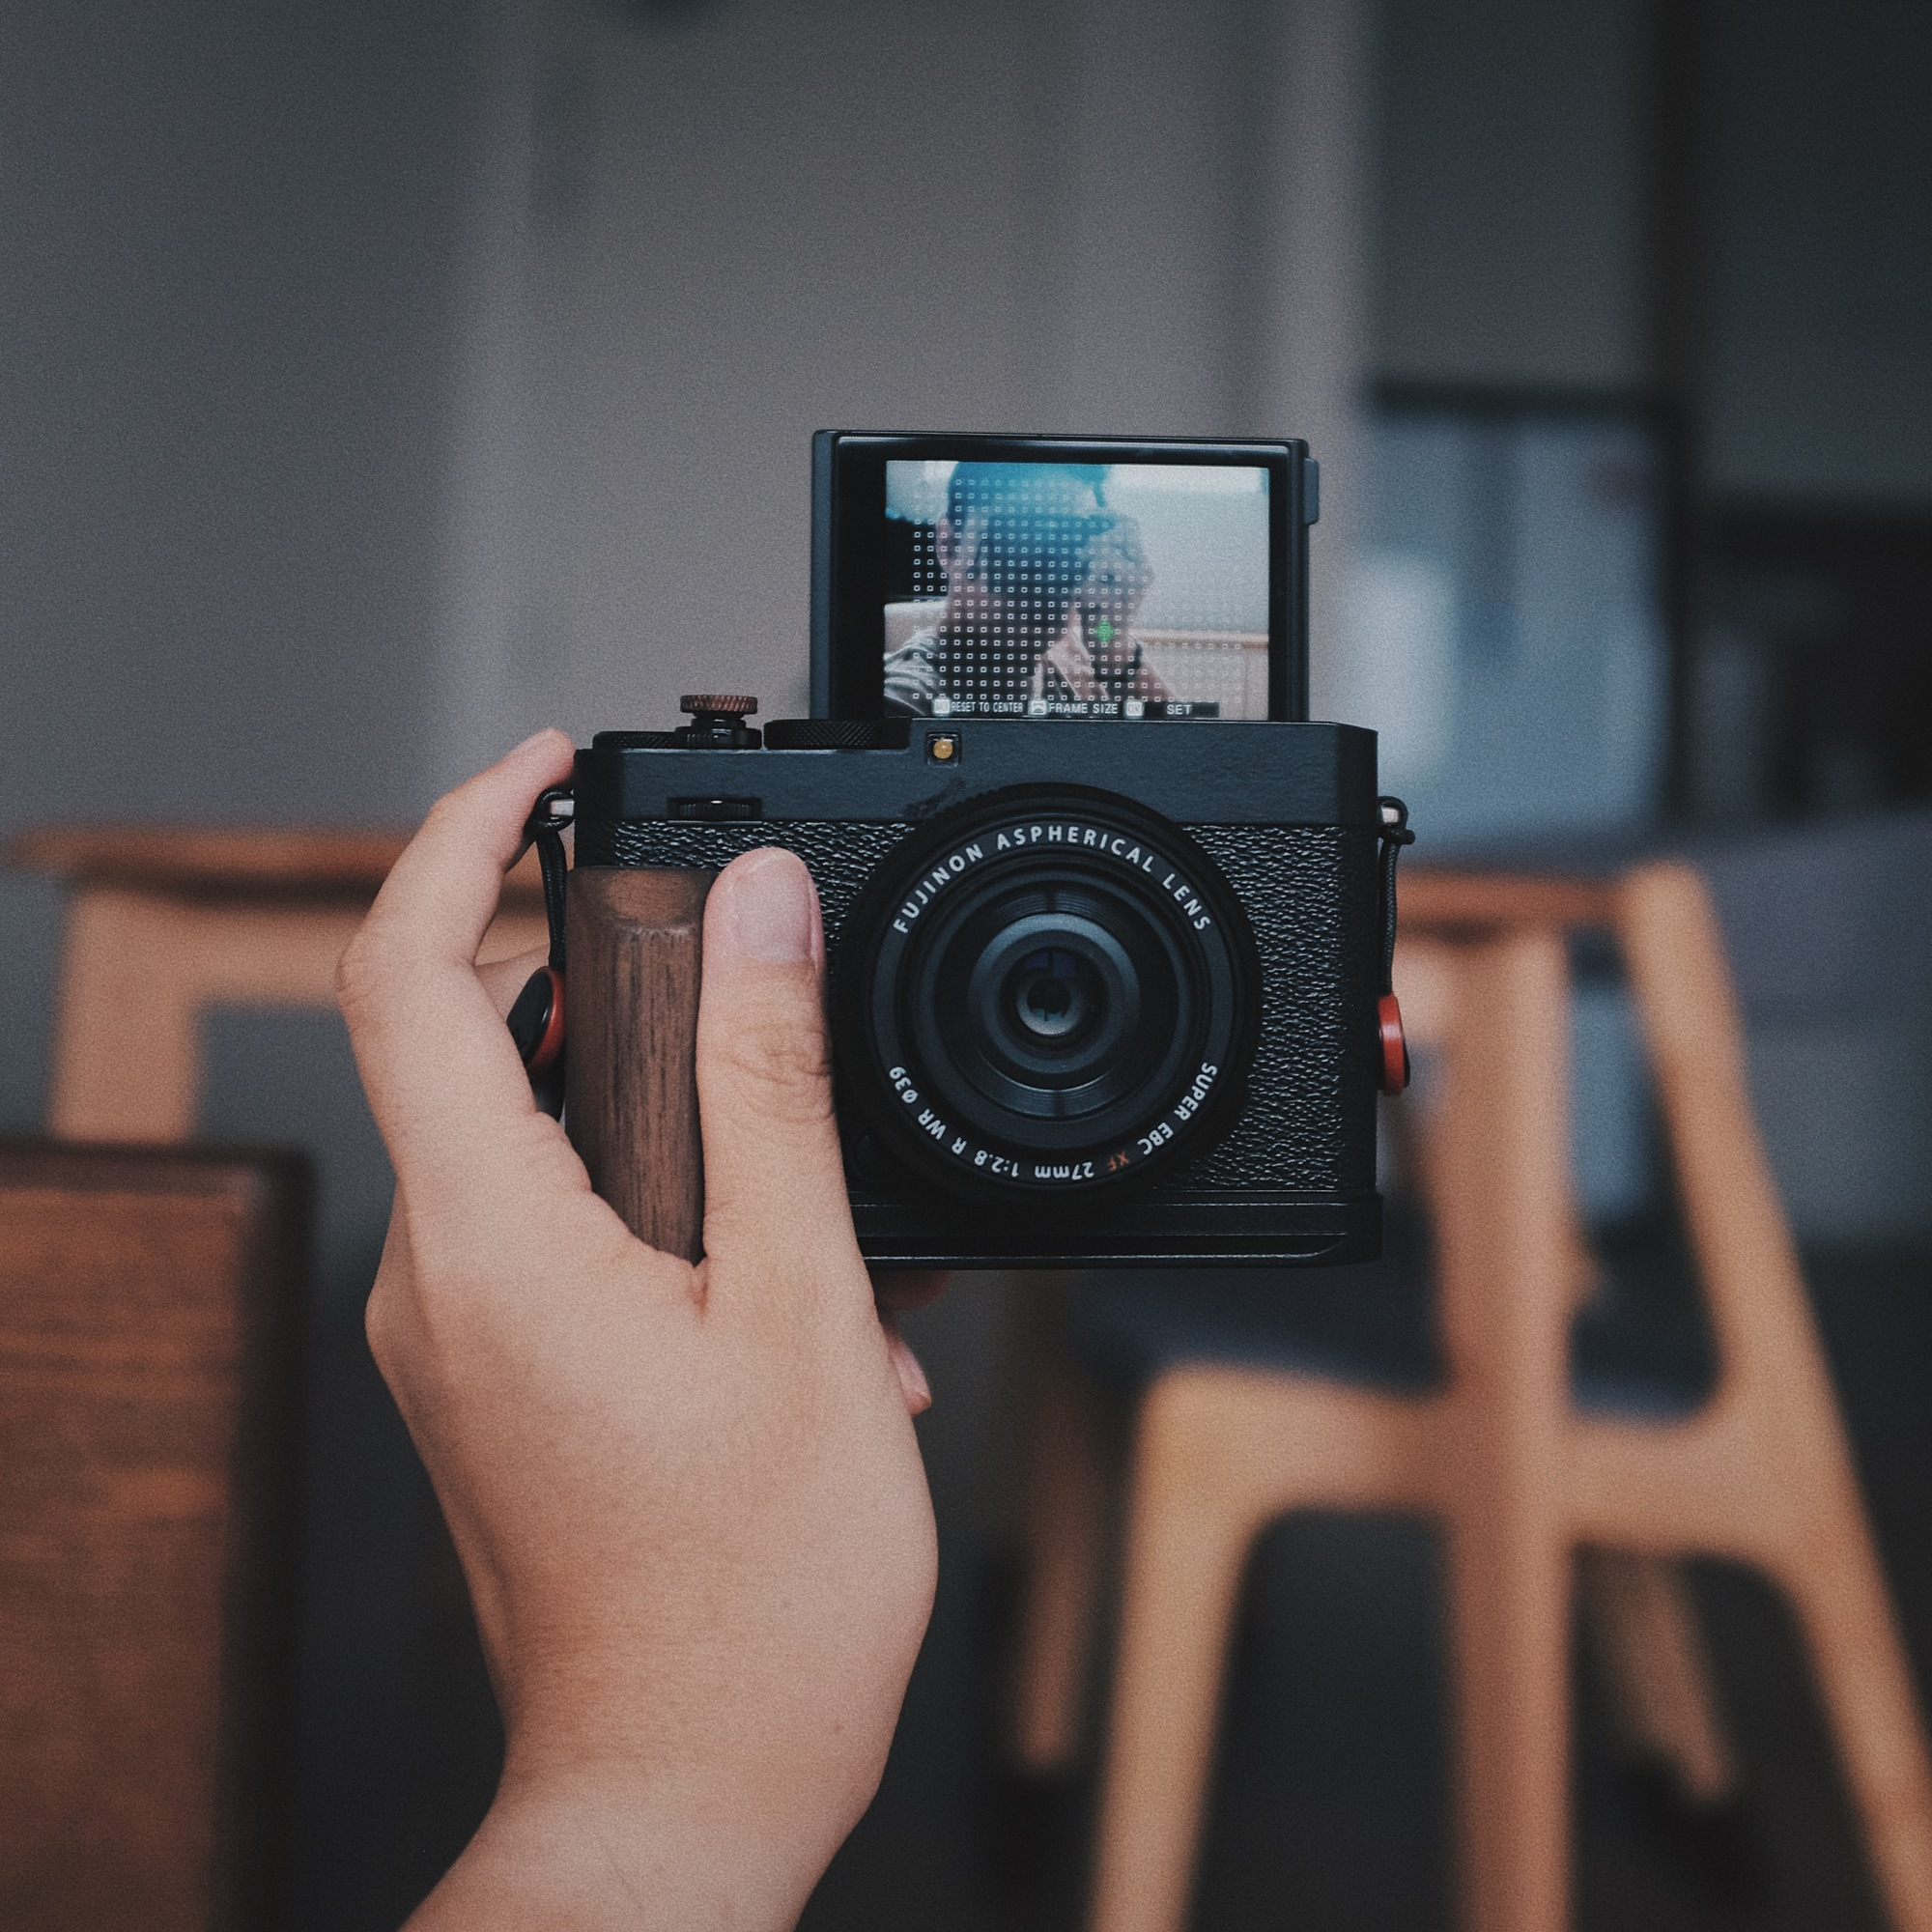
\includegraphics[width=\linewidth]{\envfinaldir/coverpic-prod.jpg}\par
            % \vskip 30pt
            \vfill

            \normalsize\rmfamily\scshape
            \copyright{} The Web Digest Project \hfill\large \envdatestr
        \end{center}
    \end{titlepage}
    % \restoregeometry
}
\newcommand{\simplehref}[1]{%
    \textcolor{blue!80!green}{\href{#1}{#1}}%
}
\renewcommand{\contentsname}{\center\Huge\sffamily\bfseries Contents\par\vskip 20pt}
\newcounter{ipartcounter}
\setcounter{ipartcounter}{0}
\newcommand{\ipart}[1]{
    % \vskip 20pt
    \clearpage
    \stepcounter{ipartcounter}
    \phantomsection
    \addcontentsline{toc}{chapter}{#1}
    % \begin{center}
    %     \Huge
    %     \sffamily\bfseries
    %     #1
    % \end{center}
    % \vskip 20pt plus 7pt
}
\newcounter{ichaptercounter}
\setcounter{ichaptercounter}{0}
\newcommand{\ichapter}[1]{
    % \vskip 20pt
    \clearpage
    \stepcounter{ichaptercounter}
    \phantomsection
    \addcontentsline{toc}{section}{\numberline{\arabic{ichaptercounter}}#1}
    \begin{center}
        \Huge
        \sffamily\bfseries
        #1
    \end{center}
    \vskip 20pt plus 7pt
}
\newcommand{\entrytitlefont}[1]{\subsection*{\raggedright\Large\sffamily\bfseries#1}}
\newcommand{\entryitemGeneric}[2]{
    % argv: title, url
    \parbox{\linewidth}{
        \entrytitlefont{#1}\par\vskip 5pt
        \footnotesize\ttfamily\mdseries
        \simplehref{#2}
    }\vskip 11pt plus 11pt minus 1pt
}
\newcommand{\entryitemGithub}[3]{
    % argv: title, url, desc
    \parbox{\linewidth}{
        \entrytitlefont{#1}\par\vskip 5pt
        \footnotesize\ttfamily\mdseries
        \simplehref{#2}\par\vskip 5pt
        \small\rmfamily\mdseries#3
    }\vskip 11pt plus 11pt minus 1pt
}
\newcommand{\entryitemAp}[3]{
    % argv: title, url, desc
    \parbox{\linewidth}{
        \entrytitlefont{#1}\par\vskip 5pt
        \footnotesize\ttfamily\mdseries
        \simplehref{#2}\par\vskip 5pt
        \small\rmfamily\mdseries#3
    }\vskip 11pt plus 11pt minus 1pt
}
\newcommand{\entryitemHackernews}[3]{
    % argv: title, hnurl, rawurl
    % \parbox{\linewidth}{
    %     \entrytitlefont{#1}\par\vskip 5pt
    %     \footnotesize\ttfamily\mdseries
    %     \simplehref{#3}\par
    %     \textcolor{black!50}{\href{#2}{#2}}
    % }\vskip 11pt plus 11pt minus 1pt
    \begin{minipage}{\linewidth}
            \entrytitlefont{#1}\par\vskip 5pt
            \footnotesize\ttfamily\mdseries
            \simplehref{#3}\par
            \textcolor{black!50}{\href{#2}{#2}}
    \end{minipage}\par\vskip 11pt plus 11pt minus 1pt
}







\begin{document}

\makeheader

\tableofcontents\clearpage




\ipart{Developers}
\ichapter{Hacker News}
\entryitemTwoLinks{Understanding Round Robin DNS}{https://news.ycombinator.com/item?id=41955912}{https://blog.hyperknot.com/p/understanding-round-robin-dns}

\entryitemTwoLinks{Open washing – why companies pretend to be open source}{https://news.ycombinator.com/item?id=41955473}{https://www.theregister.com/2024/10/25/opinion\_open\_washing/}

\entryitemTwoLinks{Should JavaScript be split into two languages?}{https://news.ycombinator.com/item?id=41955353}{https://devclass.com/2024/10/22/should-javascript-be-split-into-two-languages-new-google-driven-proposal-divides-opinion/}

\entryitemTwoLinks{New Windows driver signature bypass allows kernel rootkit installs}{https://news.ycombinator.com/item?id=41954825}{https://www.bleepingcomputer.com/news/security/new-windows-driver-signature-bypass-allows-kernel-rootkit-installs/}

\entryitemTwoLinks{Bluesky Is Not Decentralized}{https://news.ycombinator.com/item?id=41952994}{https://beige.party/@possibledog/113367977656537478}

\entryitemTwoLinks{Feds: You Don't Have a Right to Check Out Retro Video Games Like Library Books}{https://news.ycombinator.com/item?id=41952908}{https://gizmodo.com/feds-say-you-dont-have-a-right-to-check-out-retro-video-games-like-library-books-2000516767}

\entryitemTwoLinks{Show HN: Mdx – Execute your Markdown code blocks, now in Go}{https://news.ycombinator.com/item?id=41952779}{https://github.com/dim0x69/mdx}

\entryitemTwoLinks{Adventures in algorithmic trading on the Runescape Grand Exchange}{https://news.ycombinator.com/item?id=41952006}{https://tristanrhodes.com/blog/Adventures-in-Algorithmic-Trading-on-the-Runescape-Grand-Exchange}

\entryitemTwoLinks{Russia amplified hurricane disinformation to drive Americans apart}{https://news.ycombinator.com/item?id=41951773}{https://abc7chicago.com/post/russia-amplified-hurricane-disinformation-drive-americans-apart-researchers-find/15463309/}

\entryitemTwoLinks{OSI readies controversial open-source AI definition}{https://news.ycombinator.com/item?id=41951421}{https://lwn.net/SubscriberLink/995159/a37fb9817a00ebcb/}

\entryitemTwoLinks{We Can Terraform the American West}{https://news.ycombinator.com/item?id=41951420}{https://caseyhandmer.wordpress.com/2024/10/26/we-can-terraform-the-american-west/}

\entryitemTwoLinks{How can this 6 axis robot have a static accuracy of 0.05 mm? (2021) [video]}{https://news.ycombinator.com/item?id=41951408}{https://www.youtube.com/watch?v=SioCwvR\_PYY}

\entryitemTwoLinks{Before you buy a domain name, first check to see if it's haunted}{https://news.ycombinator.com/item?id=41951131}{https://www.bryanbraun.com/2024/10/25/before-you-buy-a-domain-name-first-check-to-see-if-its-haunted/}

\entryitemTwoLinks{Wikipedia article blocked worldwide by Delhi high court}{https://news.ycombinator.com/item?id=41950392}{https://en.wikipedia.org/wiki/Asian\_News\_International\_vs.\_Wikimedia\_Foundation}

\entryitemTwoLinks{Jeff Bezos killed Washington Post endorsement of Kamala Harris}{https://news.ycombinator.com/item?id=41949297}{https://www.cnbc.com/2024/10/25/jeff-bezos-killed-washington-post-endorsement-of-kamala-harris-.html}

\entryitemTwoLinks{In the US, regenerative farming practices require unlearning past advice}{https://news.ycombinator.com/item?id=41949108}{https://investigatemidwest.org/2024/10/11/regenerative-farming-practices-require-unlearning-past-advice/}

\entryitemTwoLinks{We can now fix McDonald's ice cream machines}{https://news.ycombinator.com/item?id=41949098}{https://www.ifixit.com/News/102368/victory-is-sweet-we-can-now-fix-mcdonalds-ice-cream-machines}

\entryitemTwoLinks{Company named "><SCRIPT SRC=HTTPS://MJT.XSS.HT> LTD" forced to change it (2020)}{https://news.ycombinator.com/item?id=41948666}{https://www.theguardian.com/uk-news/2020/nov/06/companies-house-forces-business-name-change-to-prevent-security-risk}

\entryitemTwoLinks{OmniParser for Pure Vision Based GUI Agent}{https://news.ycombinator.com/item?id=41948433}{https://microsoft.github.io/OmniParser/}

\entryitemTwoLinks{Federal investigators probe Tether}{https://news.ycombinator.com/item?id=41947892}{https://www.wsj.com/finance/currencies/federal-investigators-probe-cryptocurrency-firm-tether-a13804e5}\ichapter{Phoronix}
\entryitemGeneric{\hskip 0pt{}Vulkan 1.3.300 Delivers New Cooperative Matrix Extension From NVIDIA}{https://www.phoronix.com/news/Vulkan-1.3.300-Released}

\entryitemGeneric{\hskip 0pt{}Initial Intel Xe3 OpenGL \& Vulkan Driver Code Submitted For Mesa 24.3}{https://www.phoronix.com/news/Mesa-24.3-Initial-Intel-Xe3-PTL}

\entryitemGeneric{\hskip 0pt{}ASUS WMI Fix Submitted For Linux 6.12-rc5 To Handle Lunar Lake Performance Issue}{https://www.phoronix.com/news/Linux-6.12-rc5-ASUS-Platform}

\entryitemGeneric{\hskip 0pt{}Bitwarden Makes Change To Address Recent Open-Source Concerns}{https://www.phoronix.com/news/Bitwarden-Code-Cleared-Up}

\entryitemGeneric{\hskip 0pt{}KDE Fixing Many Bugs, Prepping New Plasma 6.3 Features}{https://www.phoronix.com/news/KDE-More-Fixes-Plasma-6.2.2}

\entryitemGeneric{\hskip 0pt{}Linux Adjusts "Meltdown Lite" Mitigation Handling On Newer Zen 5 CPUs}{https://www.phoronix.com/news/Meltdown-Lite-Zen-5-Linux-Fix}

\entryitemGeneric{\hskip 0pt{}Intel Core Ultra 5 245K Linux Performance}{https://www.phoronix.com/review/intel-core-ultra-5-245k-linux}

\entryitemGeneric{\hskip 0pt{}AMDGPU Changes Readied For Linux 6.13: Runtime Repartitioning, Many Fixes}{https://www.phoronix.com/news/Linux-6.13-AMDGPU-Repart}

\entryitemGeneric{\hskip 0pt{}Linux Support Continues For The Now-Canceled Snapdragon X Elite Dev Kit For Windows}{https://www.phoronix.com/news/Snapdragon-X-Elite-Dev-Kit-Goes}


\ipart{Developers~~~~(zh-Hans)}
\ichapter{Solidot}
\entryitemGeneric{\hskip 0pt{}Google DeepMind 构建 AI 帮助逆转政治极化}{https://www.solidot.org/story?sid=79596}

\entryitemGeneric{\hskip 0pt{}超新星可能清理过太阳系}{https://www.solidot.org/story?sid=79595}

\entryitemGeneric{\hskip 0pt{}人口峰值可能会更快到来}{https://www.solidot.org/story?sid=79594}

\entryitemGeneric{\hskip 0pt{}蒂姆波顿称互联网让他倍感抑郁}{https://www.solidot.org/story?sid=79593}

\entryitemGeneric{\hskip 0pt{}Kroger 和沃尔玛否认会使用数字价格标签动态定价}{https://www.solidot.org/story?sid=79592}

\entryitemGeneric{\hskip 0pt{}Linux 项目根据 OFAC 制裁名单移除俄罗斯维护者}{https://www.solidot.org/story?sid=79591}

\entryitemGeneric{\hskip 0pt{}报告称中国 5 个行业产能超过全球需求}{https://www.solidot.org/story?sid=79590}

\entryitemGeneric{\hskip 0pt{}碳排放增长速度超过了疫情前}{https://www.solidot.org/story?sid=79589}

\entryitemGeneric{\hskip 0pt{}2024 年 Salem 奖授予了 Miguel Walsh 和王艺霖}{https://www.solidot.org/story?sid=79588}

\entryitemGeneric{\hskip 0pt{}波音制造的一颗卫星在太空爆炸}{https://www.solidot.org/story?sid=79587}

\entryitemGeneric{\hskip 0pt{}Verisign 和 ICANN 更新了 DNS Root Zone 维护者服务协议}{https://www.solidot.org/story?sid=79586}

\entryitemGeneric{\hskip 0pt{}Google 开源其 AI 水印系统 SynthID}{https://www.solidot.org/story?sid=79585}

\entryitemGeneric{\hskip 0pt{}JetBrains Rider 和 WebStorm 允许非商业用户免费使用}{https://www.solidot.org/story?sid=79584}

\entryitemGeneric{\hskip 0pt{}挪威将青少年使用社交网络的最低年龄提高到 15 岁}{https://www.solidot.org/story?sid=79583}

\entryitemGeneric{\hskip 0pt{}LinkedIn 被爱尔兰数据保护机构罚款 3.1 亿欧元}{https://www.solidot.org/story?sid=79582}

\entryitemGeneric{\hskip 0pt{}香港首次发现恐龙化石}{https://www.solidot.org/story?sid=79581}

\entryitemGeneric{\hskip 0pt{}制造一个婴儿需要多少能量?}{https://www.solidot.org/story?sid=79580}

\entryitemGeneric{\hskip 0pt{}《辐射:伦敦》玩家数量突破 100 万}{https://www.solidot.org/story?sid=79579}

\entryitemGeneric{\hskip 0pt{}科学家在阿秒尺度上调查量子纠缠有多快}{https://www.solidot.org/story?sid=79578}

\entryitemGeneric{\hskip 0pt{}不受约束的私营企业如何破坏民主}{https://www.solidot.org/story?sid=79577}\ichapter{V2EX}
\entryitemGeneric{\hskip 0pt{}[问与答] 浏览器记录求指点,求帮助}{https://www.v2ex.com/t/1083950}

\entryitemGeneric{\hskip 0pt{}[程序员] 染上网瘾了怎么办?}{https://www.v2ex.com/t/1083949}

\entryitemGeneric{\hskip 0pt{}[Android] 为什么 android 机都很少有 1tb 存储的?}{https://www.v2ex.com/t/1083948}

\entryitemGeneric{\hskip 0pt{}[Android] 所以,一加 Ace3 可以解锁 BL 换 ROM 吗?}{https://www.v2ex.com/t/1083947}

\entryitemGeneric{\hskip 0pt{}[宽带症候群] 关于广东电信最近收回公网并限制 NAT4 竞技场 IP 段除了签协议还有什么方法吗?}{https://www.v2ex.com/t/1083946}

\entryitemGeneric{\hskip 0pt{}[Apple] iPad mini 为什么不每年更新了?}{https://www.v2ex.com/t/1083945}

\entryitemGeneric{\hskip 0pt{}[问与答] 考虑为 v2er 安卓客户端贡献 PR}{https://www.v2ex.com/t/1083944}

\entryitemGeneric{\hskip 0pt{}[莱卡] 雾霾}{https://www.v2ex.com/t/1083943}

\entryitemGeneric{\hskip 0pt{}[Google] gmail 收到奇怪的邮件}{https://www.v2ex.com/t/1083942}

\entryitemGeneric{\hskip 0pt{}[分享发现] Stunt Bike Extreme Online}{https://www.v2ex.com/t/1083939}

\entryitemGeneric{\hskip 0pt{}[分享创造] 职业咨询网(zhiyezixun.com)上线,专业提供一对一职业咨询服务}{https://www.v2ex.com/t/1083938}

\entryitemGeneric{\hskip 0pt{}[Apple] Paypal + 国内全币种信用卡购买美区礼品卡稳么}{https://www.v2ex.com/t/1083937}

\entryitemGeneric{\hskip 0pt{}[分享创造] 专为经常使用 JSON 数据的开发、测试、运营、产品打造的 JSON 格式化工具集合: www.jsonhome.com}{https://www.v2ex.com/t/1083936}

\entryitemGeneric{\hskip 0pt{}[服务器] 如何搭建一个内网服务 WiFi}{https://www.v2ex.com/t/1083933}

\entryitemGeneric{\hskip 0pt{}[宽带症候群] 坐标 0755,限速模板好像出问题了,是否还需要投诉}{https://www.v2ex.com/t/1083932}

\entryitemGeneric{\hskip 0pt{}[生活] 我这一生如履薄冰,你说,我能走到对岸吗?(21 岁生日总结)}{https://www.v2ex.com/t/1083931}

\entryitemGeneric{\hskip 0pt{}[问与答] 请教一下电动车 F200 和 S07 二选一选哪个?}{https://www.v2ex.com/t/1083930}

\entryitemGeneric{\hskip 0pt{}[程序员] XxlJob 迁移 SnailJob 工具来了}{https://www.v2ex.com/t/1083926}

\entryitemGeneric{\hskip 0pt{}[问与答] 省外务工的山东朋友们 会考虑 回山东(济南/青岛)买房吗?}{https://www.v2ex.com/t/1083925}

\entryitemGeneric{\hskip 0pt{}[分享创造] [分享创造] 三子棋 - 有趣的免费在线游戏}{https://www.v2ex.com/t/1083924}

\entryitemGeneric{\hskip 0pt{}[移动开发] instagram 安卓端如何抓包?}{https://www.v2ex.com/t/1083923}

\entryitemGeneric{\hskip 0pt{}[上海] 以图会友第 13 期}{https://www.v2ex.com/t/1083921}

\entryitemGeneric{\hskip 0pt{}[问与答] i3 10100f 升级到 i5 9400f 能解决 cpu 不够吗?}{https://www.v2ex.com/t/1083920}

\entryitemGeneric{\hskip 0pt{}[问与答] 大家坐保友金豪 B 体验如何?}{https://www.v2ex.com/t/1083918}

\entryitemGeneric{\hskip 0pt{}[Windows] 搜狗输入法脸都不要了}{https://www.v2ex.com/t/1083917}

\entryitemGeneric{\hskip 0pt{}[问与答] 翻到一个以前的红米 6a,不知道能不能刷成常规 Linux 用?}{https://www.v2ex.com/t/1083916}

\entryitemGeneric{\hskip 0pt{}[路由器] 求一款路由器设备, 4G/5G 转 Wi-Fi,但可以刷机}{https://www.v2ex.com/t/1083915}

\entryitemGeneric{\hskip 0pt{}[推广] Python 潮流周刊\#74:创下吉尼斯世界记录的 Python 编程课(摘要)}{https://www.v2ex.com/t/1083914}

\entryitemGeneric{\hskip 0pt{}[生活] 求推荐收听国外广播的 app}{https://www.v2ex.com/t/1083912}

\entryitemGeneric{\hskip 0pt{}[Linux] 想咨询下 TN133A2 怎么样}{https://www.v2ex.com/t/1083911}

\entryitemGeneric{\hskip 0pt{}[远程工作] [remote/头部交易所] Web 开发工程师}{https://www.v2ex.com/t/1083909}

\entryitemGeneric{\hskip 0pt{}[V2EX] v2ex 算不是算是仅剩的中文稍微好点的 IT 类论坛了}{https://www.v2ex.com/t/1083908}

\entryitemGeneric{\hskip 0pt{}[问与答] 没有 visa 卡怎么注册 azure,需要使用 bing search api}{https://www.v2ex.com/t/1083907}

\entryitemGeneric{\hskip 0pt{}[问与答] 有用 AirPods4 的朋友吗}{https://www.v2ex.com/t/1083906}

\entryitemGeneric{\hskip 0pt{}[问与答] 很喜欢 iMac 2012 的 1080p 镜面屏,买个普通镜面屏显示器能平替吗}{https://www.v2ex.com/t/1083905}

\entryitemGeneric{\hskip 0pt{}[Apple] 美区 Apple One Premier 开车价格}{https://www.v2ex.com/t/1083904}

\entryitemGeneric{\hskip 0pt{}[远程工作] [remote/头部交易所] 测试工程师}{https://www.v2ex.com/t/1083903}

\entryitemGeneric{\hskip 0pt{}[问与答] 一张 5 亿条数据的表,命中索引后扫描 1~10 行数据,请问在命中索引的情况下查询消耗时长大概多少?}{https://www.v2ex.com/t/1083902}

\entryitemGeneric{\hskip 0pt{}[分享发现] 搞了一个小工具, remove color from image}{https://www.v2ex.com/t/1083901}

\entryitemGeneric{\hskip 0pt{}[Apple] 求推荐,有没有像 Mac M 芯片一样,几乎听不到风扇转的 Windows 电脑?}{https://www.v2ex.com/t/1083900}

\entryitemGeneric{\hskip 0pt{}[Apple] mac mini m2 外接两屏幕无法息屏了}{https://www.v2ex.com/t/1083899}

\entryitemGeneric{\hskip 0pt{}[Apple] 苹果图书有没有可能使用 AI 朗读其内容并自动翻页?}{https://www.v2ex.com/t/1083897}

\entryitemGeneric{\hskip 0pt{}[远程工作] [remote/头部交易所] 合约- Java 开发工程师}{https://www.v2ex.com/t/1083896}

\entryitemGeneric{\hskip 0pt{}[分享创造] QQ 电脑版自动抢红包插件}{https://www.v2ex.com/t/1083895}

\entryitemGeneric{\hskip 0pt{}[OpenAI] 大家在使用哪些可以用自定义 api 的 AI 应用?}{https://www.v2ex.com/t/1083894}

\entryitemGeneric{\hskip 0pt{}[问与答] 双十一什么时候买 iPhone 最便宜?}{https://www.v2ex.com/t/1083893}

\entryitemGeneric{\hskip 0pt{}[投资] 手痒打算去为韭菜添砖加瓦,哪个平台好?}{https://www.v2ex.com/t/1083891}

\entryitemGeneric{\hskip 0pt{}[问与答] 感觉运气特别差,有没有什么可以转运的小首饰?}{https://www.v2ex.com/t/1083890}

\entryitemGeneric{\hskip 0pt{}[酷工作] [广州-三七互娱-社招-非技术岗位-可以推荐给女伴]资深财务 BP、中/高级福利规划、HRBP、高级薪酬绩效、高级培训讲师、高级组织发展、总裁助理}{https://www.v2ex.com/t/1083889}

\entryitemGeneric{\hskip 0pt{}[前端开发] 有没有技术博主讲课很全面的?}{https://www.v2ex.com/t/1083888}


\ipart{Generic News}
\ichapter{Reuters}
\entryitemWithDescription{\hskip 0pt{}Russian attacks prompts Ukraine's Zelenskiy to ask allies for more resolve}{https://www.reuters.com/world/europe/russian-attacks-prompts-ukraines-zelenskiy-ask-allies-more-resolve-2024-10-26/}{A string of Russian attacks killed and injured civilians in widely separated parts of Ukraine, prompting President Volodymyr Zelenskiy to issue a new call to Kyiv\textquotesingle s allies on Saturday to intensify pressure on...}

\entryitemWithDescription{\hskip 0pt{}Thousands protest in Lisbon against police violence}{https://www.reuters.com/world/europe/thousands-protest-lisbon-against-police-violence-2024-10-26/}{Thousands of people took to the main avenue of downtown Lisbon on Saturday to protest police violence, several days after a policeman shot a Cape Verde-born Portuguese resident, triggering a wave of...}

\entryitemWithDescription{\hskip 0pt{}Vatican summit praises women's leadership, but stops short on women clergy}{https://www.reuters.com/world/europe/vatican-summit-praises-womens-leadership-stops-short-women-clergy-2024-10-26/}{A major Vatican summit of global Catholic leaders ended on Saturday with a call for women to be granted more leadership roles in the Church but stopped short of calling for women to be ordained as...}

\entryitemWithDescription{\hskip 0pt{}Israeli military eases some safety restrictions for parts of northern Israel}{https://www.reuters.com/world/middle-east/israeli-military-eases-some-safety-restrictions-parts-northern-israel-2024-10-26/}{Israel\textquotesingle s military eased some safety restrictions for residents in areas of northern Israel late on Saturday, a possible indication that it does not expect any immediate large-scale attack from Iran or its proxies in the...}

\entryitemWithDescription{\hskip 0pt{}Georgian ruling party wins majority in election with 70\% of precincts counted, official results say}{https://www.reuters.com/world/europe/georgian-ruling-party-wins-majority-election-with-70-precincts-counted-official-2024-10-26/}{Georgia\textquotesingle s ruling Georgian Dream party won 53\% of the vote in a parliamentary election on Saturday, with 70\% of precincts counted, the central electoral commission...}

\entryitemWithDescription{\hskip 0pt{}Bus crash in central Mexico kills 19 people}{https://www.reuters.com/world/americas/two-dozen-people-die-central-mexico-bus-crash-2024-10-26/}{Nineteen people died and six others were injured when a bus crashed on a highway in Mexico\textquotesingle s central state of Zacatecas on Saturday, local authorities...}

\entryitemWithDescription{\hskip 0pt{}Ghana rejects Reuters report on jihadis finding refuge in its north}{https://www.reuters.com/world/africa/ghana-rejects-reuters-report-jihadis-finding-refuge-its-north-2024-10-26/}{Ghana\textquotesingle s government on Saturday rejected Reuters reporting on Islamist militants in Burkina Faso that found they are discreetly using neighbouring Ghana\textquotesingle s north as a logistical and medical base to sustain...}

\entryitemWithDescription{\hskip 0pt{}At least 124 killed after Sudan's RSF attack village, activists say}{https://www.reuters.com/world/africa/least-124-killed-after-sudans-rsf-attack-village-activists-say-2024-10-26/}{Sudan\textquotesingle s paramilitary Rapid Support Forces (RSF) killed at least 124 people in a village in El Gezira State on Friday, activists said, in one of the deadliest incidents of an 18-month war and largest in a spate of attacks...}

\entryitemWithDescription{\hskip 0pt{}Israeli army leaves north Gaza hospital, detains medics, says health ministry}{https://www.reuters.com/world/middle-east/israeli-army-leaves-north-gaza-hospital-detains-medics-says-health-ministry-2024-10-26/}{Footage circulated by the health ministry showed damage to several...}

\entryitemWithDescription{\hskip 0pt{}Germany's Scholz urges Iran to de-escalate after Israeli strikes}{https://www.reuters.com/world/europe/germanys-scholz-urges-iran-de-escalate-after-israeli-strikes-2024-10-26/}{German Chancellor Olaf Scholz called on Iran to end the cycle of escalation following Israeli strikes on Iranian military sites early on Saturday, saying restraint could pave the way for peace in the Middle...}

\entryitemWithDescription{\hskip 0pt{}Italy police arrest four over alleged illegal database access, source says}{https://www.reuters.com/world/europe/italy-police-arrest-four-over-alleged-illegal-database-access-source-says-2024-10-26/}{Italian police have placed four people under house arrest including Leonardo Maria Del Vecchio, son of the late billionaire founder of Luxottica, as part of a probe into alleged illegal access to state databases, a source said on...}

\entryitemWithDescription{\hskip 0pt{}Ten Iranian border guards killed in attack near southeastern border}{https://www.reuters.com/world/middle-east/ten-iranian-border-guards-killed-attack-southeast-ministry-says-2024-10-26/}{Ten Iranian border guards were killed in an attack in restive southeastern Iran on Saturday, state media quoted the interior ministry as saying, in the latest clash with suspected Sunni Muslim...}

\entryitemWithDescription{\hskip 0pt{}Sixty years after the unwinding of Jim Crow, a historic US election}{https://www.reuters.com/world/us/sixty-years-after-unwinding-jim-crow-historic-us-election-2024-10-26/}{It's almost at the edge of living memory: President Lyndon Johnson signing the Civil Rights Act in July 1964, urging Americans to ``close the springs of racial...}






\clearpage
\leavevmode\vfill
\footnotesize

Copyright \copyright{} 2023-2024 Neruthes and other contributors.

This document is published with CC BY-NC-ND 4.0 license.

The entries listed in this newsletter may be copyrighted by their respective creators.

This newsletter is generated by the Web Digest project.

The newsletters are also delivered via Telegram channel \CJKunderline{\href{https://t.me/webdigestchannel}{https://t.me/webdigestchannel}}.\\
RSS feed is available at \CJKunderline{\href{https://webdigest.pages.dev/rss.xml}{https://webdigest.pages.dev/rss.xml}}.

This newsletter is available in PDF at
\CJKunderline{\href{https://webdigest.pages.dev/}{https://webdigest.pages.dev/}}.

The source code being used to generate this newsletter is available at\\
\CJKunderline{\href{https://github.com/neruthes/webdigest}{https://github.com/neruthes/webdigest}}.

This newsletter is also available in
\CJKunderline{\href{http://webdigest.pages.dev/readhtml/\envyear/WebDigest-20241027.html}{HTML}} and
\CJKunderline{\href{https://github.com/neruthes/webdigest/blob/master/markdown/\envyear/WebDigest-20241027.md}{Markdown}}.


\coverpic{https://unsplash.com/photos/a-view-of-a-mountain-range-with-trees-in-the-foreground-lYHT5fthhzM}{Jacob Grishey}


\end{document}
